%!TEX root = thesis.tex

\chapter{Motion planning}
\label{chap:moveit}
This chapter explains the motion planning related part of the thesis. The introduction gives an overview about motion planning problems in general. Further on, the sampling based motion planning approach is described. Subsequent sections explain the integration of the motion planning framework \emph{MoveIt} into the existing robot setup.

\section{Introduction}

\citep[p. 1--11]{choset2005} describes motion planning as to be the task of finding a collision free path from one robot \emph{configuration} to another one. The classic path planning problem is the so called \emph{piano mover's problem}, originally mentioned by \cite{schwartz1983}. It is assumed to have a piano, which states a three dimensional rigid body and a set of known obstacles. The problem is to find a continuous motion that moves the piano from its current position to a given target position without touching any of the obstacles. Thereby the piano can freely be moved and rotated in Cartesian space. 

A generalized version of the \emph{piano mover's problem} is to find paths for a robot, composed from a set of rigid bodies, linked by joints while enforcing \emph{constraints} during that motions. A \emph{constraint} could be to avoid obstacles or to keep the robot's end effector in an upright position. Therefore it is important to have a representation of a robot's state that allows to determine the location of all robot parts. This representation is called the \emph{configuration} of a robot and the \emph{configuration space} is the set of all possible configurations, the robot is able to acquire. The dimension of the configuration space is the amount of \emph{degrees of freedom} (DOF), which is the number or independent variables that are necessary to describe a configuration. An imaginary free flying piano has six degrees of freedom as its configuration consists of the position and orientation $(x,y,z,roll,pitch,yaw)$ in Cartesian space. A robot arm with 7 joints has 7 degrees of freedom and its configuration are the joint positions. The motion planning problem is to find a path in the configuration space that connects start and goal configuration without violating constraints. This is a very complex problem and there exist various different approaches to find solutions. Examples are among others the \emph{bug algorithms}\citep[chapter 2]{choset2005}, \emph{potential functions}\citep[chapter 4]{choset2005} or \emph{sampling-based methods}\citep[chapter 7]{choset2005}. As the solution within this project only uses sampling based algorithms, a short overview about this class of methods will be given in the following section.

\section{Sampling-based motion planning}

Based on \citep[chapter 2]{omplPrimer}, sampling-based motion planning can be seen as a concept, capable of handling planning problems efficiently, especially for systems with many degrees of freedom. The general idea is to generate a set of random sample points that are uniformly distributed in the configuration space of the robot and then connect start and goal state by connecting the samples via collision free paths, with respect to possible motion constraints. Those methods are usually faster than traditional approaches because it is not necessary to reason about the whole configuration space but only about a finite number of sample configurations. The majority of sampling-based approaches are known to be \emph{probabilistic complete}, which means that the probability of finding an existing solution tends to 1 as the number of sample points increases to infinity. But they are not able to decide if a valid solution exists at all. The following definitions are used throughout this section to describe the concepts of sampling-based motion planning.

\begin{itemize}

\item \textbf{State space} \\
The \emph{state space} $\mathcal{S}$ is equal to the configuration space and consists of all possible robot configurations (states).

\item \textbf{Free state space} \\
The \emph{free state space} $\mathcal{S}_{free}$ is a subset of $\mathcal{S}$, containing only collision free states.  

\item \textbf{Path} \\
A \emph{path} is a sequence of states. If each state within the path is contained in $\mathcal{S}_{free}$, it is called a \emph{collision free} path.  

\end{itemize}

The sampling-based motion planners can be categorized into two major types - \emph{probabilistic roadmaps} (PRM) and \emph{tree-based planners}. Common to both methods is that they create uniformly distributed samples within the free state space. As the shape of $\mathcal{S}_{free}$ is not explicitly known, the created sample states are checked for collisions before using them. The following paragraphs give a short overview about both approaches.

\paragraph{Probabilistic roadmaps}

That approach uses the sampled states to create a ``roadmap'' of the free state space. Therefore each sample point is connected to an amount of $k$ nearby sample points via collision free paths. This is done by a local planner that simply interpolates between two points in the desired resolution while watching out for collisions. If no collision is detected, a new edge is introduced into the graph that is formed by the roadmap. After completing the graph, a planning query can be reduced to finding the shortest path within that graph that connects the start state and the goal state (figure \ref{fig:sampling_based}a).

\paragraph{Tree-based planners}

A lot of different sampling-based planning algorithm are using the tree based approach, as there are for example (RRT, EST, SBL or KPIECE). The difference to PRM is that this method uses a tree data structure of the free state space, which means that the resulting graph contains no cycles. The root of the tree is the start state and the tree is then expanded towards the goal state by creating collision free connections between sample points. If the goal is reached, the solution is found (figure \ref{fig:sampling_based}b). The different approaches differ in the strategy that is used to expand the tree towards the goal state.\\

\begin{figure}[ht]
	\centering
  	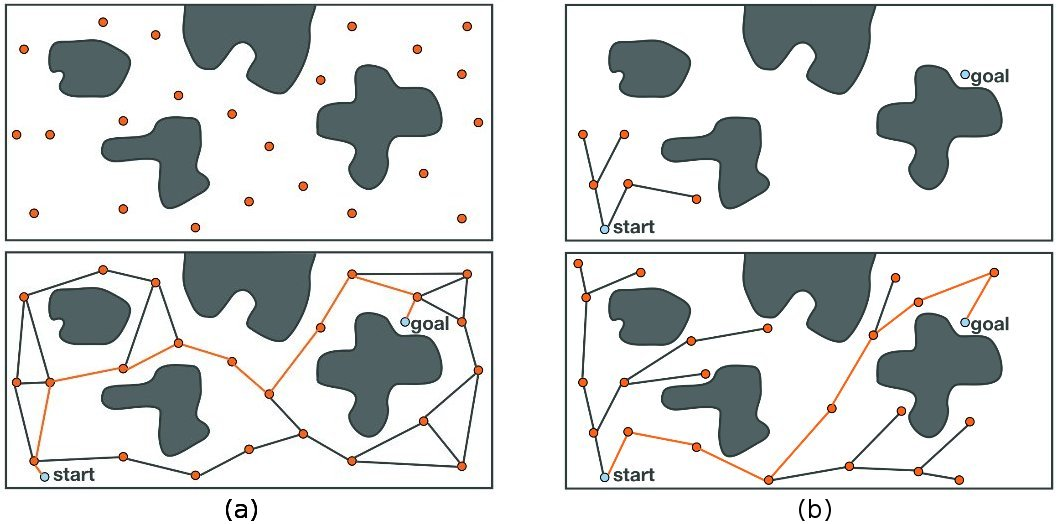
\includegraphics[width=1.0\textwidth]{images/sampling_based.jpg}
	\caption[Sampling based algorithms]{Probabilistic roadmap (left) and tree based approach (right)}
	{\scriptsize Image source: \citep{omplPrimer}}
	\label{fig:sampling_based}
\end{figure}

Generally can be said that the tree based approaches are more adequate for \emph{single query planning} because the tree usually does not has to cover the whole free state space. A roadmap could be reused for subsequent queries. As the most methods also require the search of a nearest neighbour, the utilized distance metric is also a crucial part within sampling-based motion planning as it is not always easy to identify the optimal method for finding nearby states in systems with large degrees of freedom.  

\section{The MoveIt motion planning framework}

\begin{figure}[ht]
	\centering
	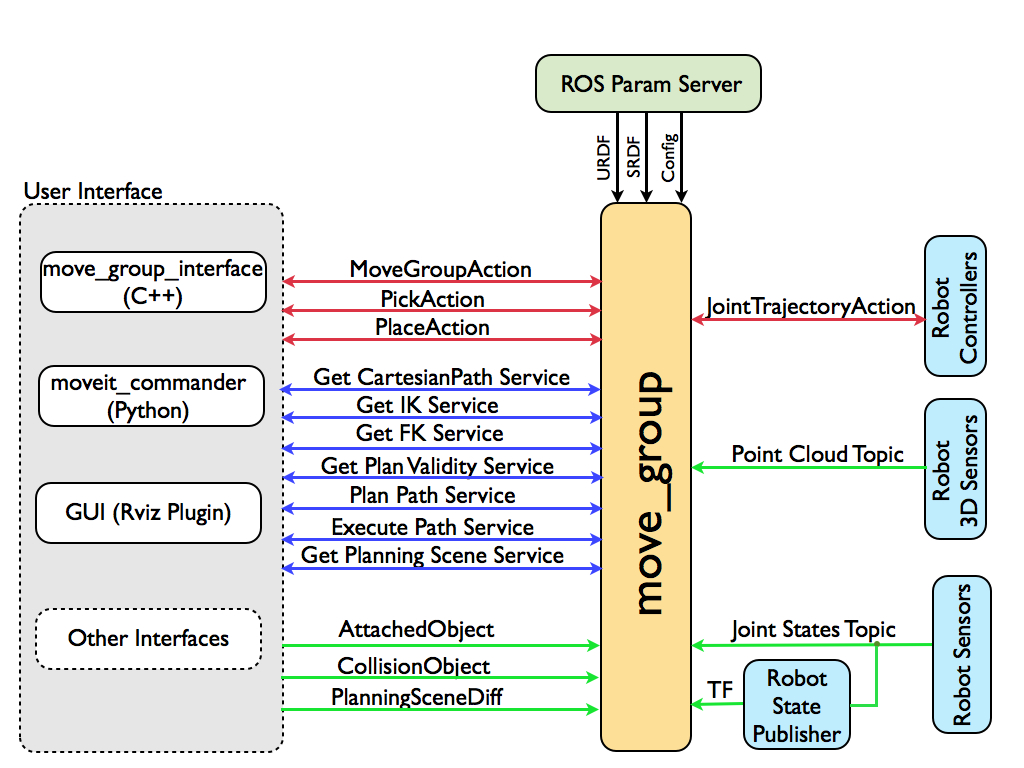
\includegraphics[width=0.75\textwidth]{images/moveit_architecture.jpg}
	\caption[Moveit architecture]{MoveIt architecture}
	{\scriptsize Image source: \url{http://moveit.ros.org/documentation/concepts}}
	\label{fig:moveit_arch}
\end{figure}

This section gives an overview about MoveIt's system architecture and introduces basic concepts. MoveIt\citep{MoveIt} is an open source framework for motion planning that is fully integrated into ROS. MoveIt was originally developed by Willowgarage\footnote{http://www.willowgarage.com} but since April 2012 it is maintained by the Open Source Robotics Foundation (OSRF). Figure \ref{fig:moveit_arch} gives an overview about the system architecture. \\

Central part of the framework is the \path{move_group} node. Configuration of that node happens via the parameter server. Therefore it is necessary to create a MoveIt configuration package. This is a ROS package that contains a description of the robot setup along with a number of necessary configuration files. The creation of that package and the necessary configuration steps are described in section \ref{sec:moveit_assistant}. The \path{move_group} node maintains a \emph{planning scene} which is an internal representation of the world. This planning scene bases on a kinematic description of the robot in the URDF format, which is a special markup language, designed to describe robots. The necessary steps to create that URDF description for our robot setup are explained in section \ref{sec:urdf}. \\

On top of this static description the \path{move_group} node needs to keep track of the current state of the robot. Therefore it expects the actual joint states to be published to a topic named \path{joint_states}. If there are additional objects within the robot's workspace that are not part of the robot description, they also have to be added to the planning scene. This can be done either by explicitly adding them via the corresponding topics (\path{CollisionObject} or \path{PlanningSceneDiff}) or by integrating information from 3D sensors like Kinect cameras. This information will then be taken into account during motion planning and collisions are avoided. But some collisions are intended. For example if an object has to be picked up, the gripper has to get in contact to this object. That means, collision checking for specific objects has to be (temporary) disabled to allow those controlled collisions. Therefore the \path{move_group} node maintains a so called \path{AllowedCollisionMatrix} to which objects can be added or removed. This also happens via the \path{PlanningSceneDiff} topic. \\

The \path{move_group} node provides a ROS interface, consisting of various ROS topics and services that allow to access its functionality. The services \path{GetIKService} and \path{GetFKService} can be used to solve inverse and forward\footnote{The problem of computing the end effector position in Cartesian space for a given robot configuration} kinematics problems. The \path{PlanPathService} handles motion planning requests and the \path{ExecutePathService} can be used to execute the planned trajectories on the connected hardware. Additionally there are the \path{PickAction} and \path{PlaceAction} servers available. Those action servers are intended to plan and execute all stages of pick and place operations. They were utilized in the benchmark pick and place task that was implemented in the scope of this project. Their usage is therefore described in chapter \ref{chap:pick_place}. \\

The functionality of the \path{move_group} node can be accessed in different ways. One way is to directly use the previously described services of the ROS interface. Another way is to use the \path{move_group_interface} which is a C++ wrapper around that ROS interface or the corresponding Python wrapper (\path{moveit_commander}). MoveIt also provides a planning plugin for the RViz visualization tool which can be used to do planning requests based on a graphical user interface. \\

The planning outcome of MoveIt is a time parametrized trajectory consisting of a set of waypoints. A waypoint is a joint configuration, described by the tuple $(p,v,a,t)$ where $p \in \mathbb{R}^n$ are the positions, $v \in \mathbb{R}^n$ the velocities and $a \in \mathbb{R}^n$ the accelerations at time $t$ and $n$ is the number of involved joints. Those waypoints mark the important points along the path, the manipulator has to move. Connecting  MoveIt to the hardware requires therefore controllers that are able to translate such time parametrized trajectories into a sequence of suitable motor commands. Just sending the joint positions within the waypoints to the robot would not suffice as a trajectory is also constrained in terms of \emph{velocities} and \emph{accelerations} over \emph{time}. Therefore the controller needs to be able to interpolate between the subsequent waypoints and calculate intermediate joint positions based on the loop rate of the control cycle. Section \ref{sec:hardware_adapter} explains in detail how this problem was solved and how the connection to the (simulated or real) hardware was established.\\

Various important parts of MoveIt are implemented as plugins which means they are replaceable by other components that provide the same interface. The inverse kinematics plugin we utilized uses the Kinematics and Dynamics Library\footnote{http://www.orocos.org/kdl} (KDL) for solving IK problems. The planning plugin provides access to the sampling based planners of the  Open Motion Planning Library\footnote{http://ompl.kavrakilab.org} (OMPL), which is a framework that contains implementations of many different motion planning algorithms. Therefore it is possible to choose, which one of those algorithms to use during planning requests. \\

\section{Creating the URDF model of the robot setup}
\label{sec:urdf}

The \emph{Unified Robot Description Format} (URDF) is a markup language, designed to describe robots. The description happens in text files, in a special XML format. The most important elements in the XML specification\footnote{http://wiki.ros.org/urdf/XML} are:

\begin{itemize}

\item \textbf{link} \\
Describes the all necessary properties of a specific robot link. Each link must have a unique name. The visual, inertial and collision details are configured in the corresponding subtags of the link element. The visual part as well as the collision model can either be composed from primitive shapes
or from mesh files. If mesh files are used it is important that they are not to complex. Especially for the collision model it is recommended to use a simplified model to avoid a performance loss because during planning requests there happens a lot of collision checking.

\item \textbf{joint} \\
Describes the properties of a joint. A joint is a flexible connection between two links, having exactly one parent and one child link. Each joint states a new reference frame for its child link and it is positioned relative to its parent frame. The joint actuates its child link relative to its parent link along the joint axis. There are different types of joints available but for the current project only \emph{fixed} and \emph{revolute} joints are of interest. A fixed joint states a rigid connection between parent and child link. A revolute joint is a rotational joint with one degree of freedom. Details like angular joint limits, axis orientation and the dynamic properties of the joint motors can be configured in the corresponding subtags of the joint element.

\end{itemize}
\begin{figure}[ht]
	\centering
  	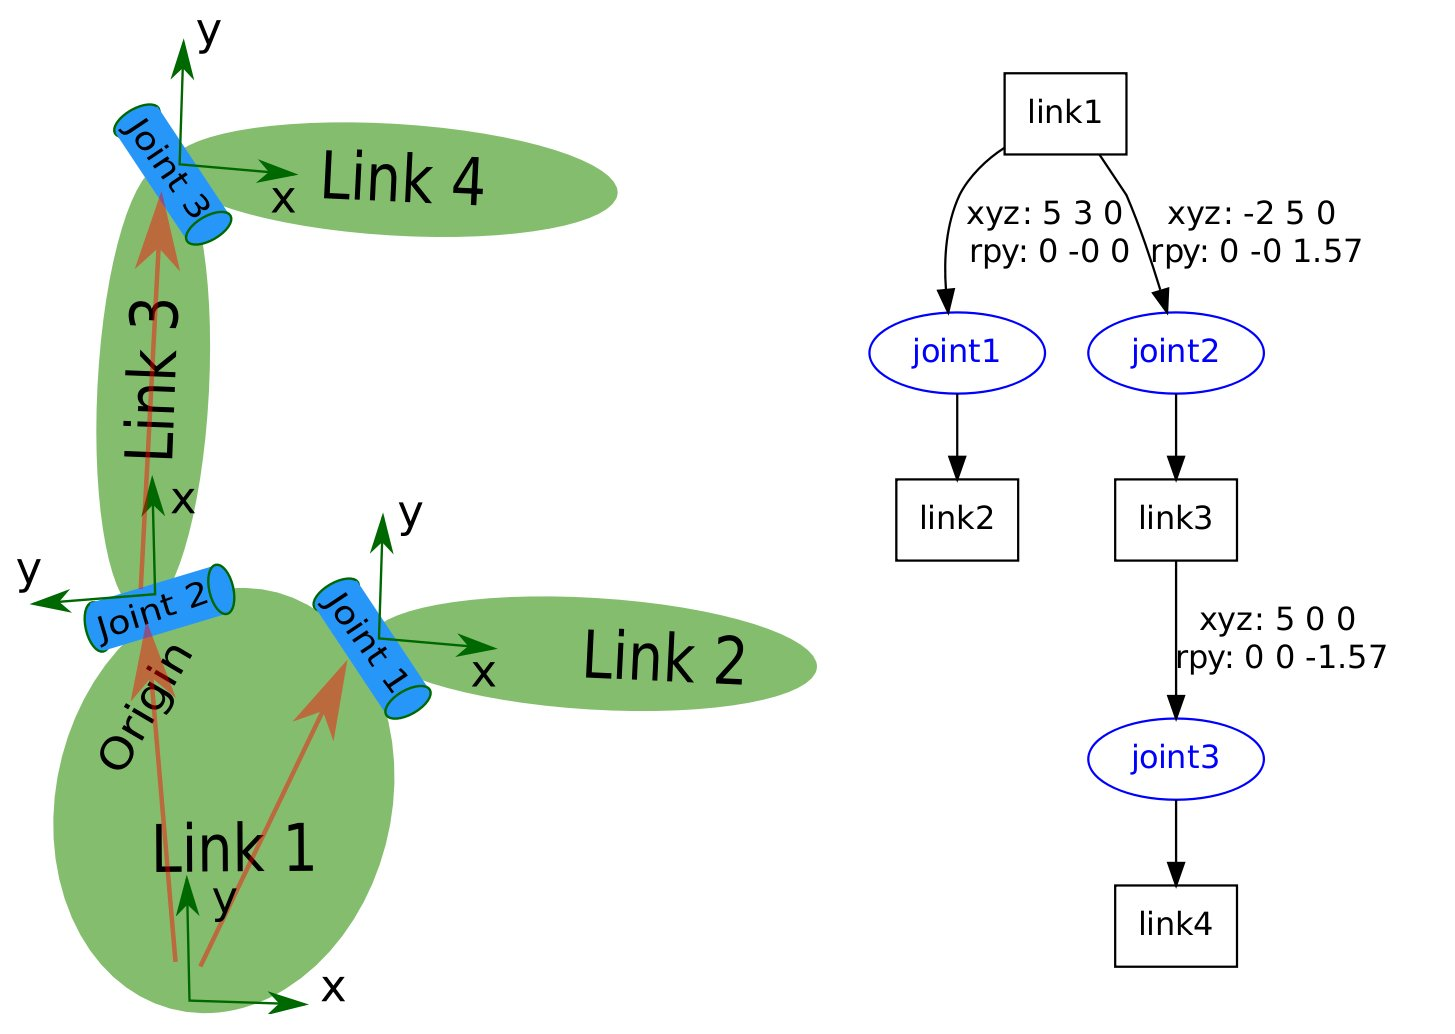
\includegraphics[width=0.75\textwidth]{images/urdf_chain.jpg}
	\caption[URDF graph]{URDF graph}
	{\scriptsize Image source: http://wiki.ros.org/urdf/Tutorials/Create your own urdf file}
	\label{fig:urdf_graph}
\end{figure}
Those elements are used to form the URDF graph that exactly describes the kinematic chain of the robot components and their placement relative to each other. A simple example for such a graph is visualized in figure \ref{fig:urdf_graph}. This description can get very large as a lot of different components are involved. So it is possible to organize it into a set of text files, each one describing one part of the whole. For example one file could describes a robot arm. Other files can then use that description and insert multiple instances of that arm into the setup. The \texttt{xacro} ROS package provides the necessary functionality to combine all those text files into one XML string. \emph{XACRO} stands for \emph{XML Macro} and is designed to parse xacro files and combine them into one single XML document, containing the resulting URDF description.\\

The URDF description of the IIS robot setup is spread across multiple packages, located in the \path{iis_hardware} directory of the \path{iis_robot_sw} repository. Arm and gripper descriptions are located in seperate packages (\path{lwr_description} and \path{schunk_description}), the \path{iis_robot} package brings all the components together. The description of the Schunk SDH gripper was taken from the \path{schunk_description} ROS package. The model of the KUKA LWR arm was adapted from the Github repository\footnote{https://github.com/RCPRG-ros-pkg/lwr\_robot/tree/hydro-devel/lwr\_defs} of the \emph{Robot Control and Pattern Recognition Group}\footnote{University of Warsaw (http://robotyka.ia.pw.edu.pl/twiki/bin/view/Main)}. The other parts of the model, namely the robot torso and the table had to be created. The descriptions are located in a seperate files within the \texttt{uibk\_robot} package (\texttt{torso.xacro} and \texttt{table.xacro}). \\

\begin{figure}[h]
	\centering
  	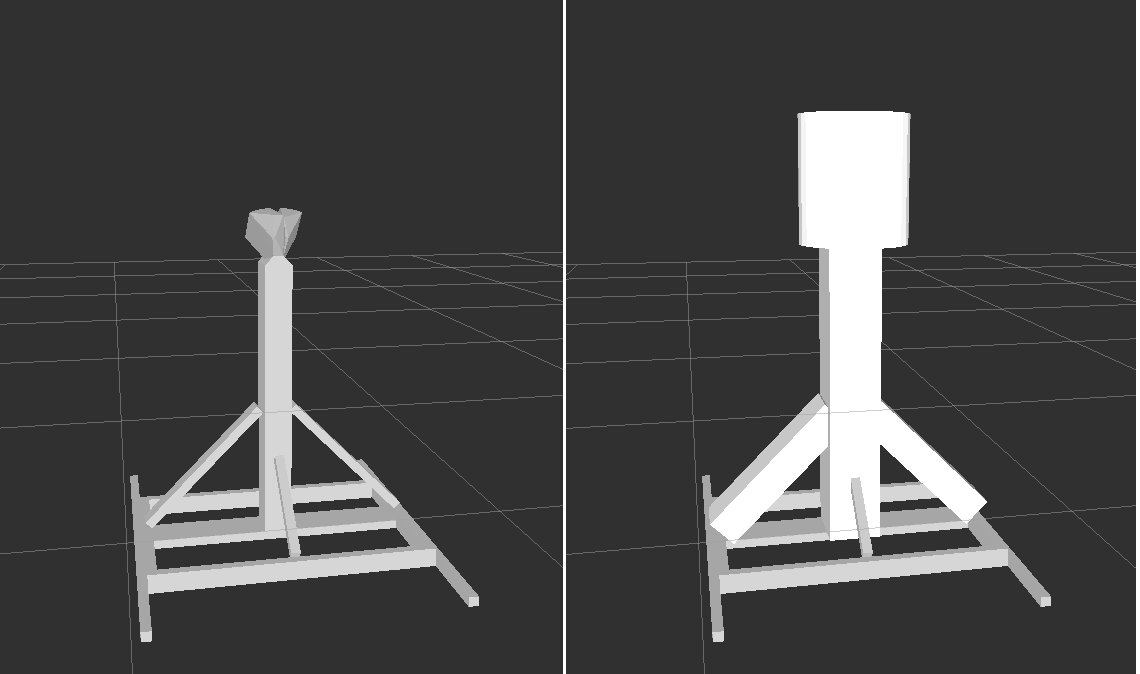
\includegraphics[width=1.0\textwidth]{images/torso.jpg}
	\caption{Visual and collidable model of torso}
	\label{fig:torso_col}
\end{figure}

The mesh files, used in the description of the robot torso have been exported from the V-Rep simulation scene. For the visual part we took the mesh as it is. For the collision geometry we created an increased version of the original mesh to provide a safety padding of 2.5 cm around the torso links. Moreover a cylinder with a diameter of 40 cm was added in the head area to ensure that the planner avoids accidental hits in the region where the Kinect camera is mounted. Figure \ref{fig:torso_col} shows the visual (left image) and the collidable (right image) part of the torso model. \\

The table was modelled from primitive shapes. We designed the XML structure of the table description in a way that allows to easily adjust the size of the table, as can bee seen in listing \ref{lst:table}. The collision geometry of the table is also slightly larger than the visual part to provide safety margins. \\

\lstset{language=XML,style=customxml}
\begin{minipage}{\linewidth}
\begin{lstlisting}[caption={XML snippet, inserting the table model into the URDF}, label=lst:table]
<!-- draw the table relative to the origin -->
<xacro:model_table name="table" 
	     parent="world"
	     length="2.22"
	     width="0.8">
	<!-- Place the table relative to the world reference frame -->
	<origin xyz="-0.029 -0.3 0" />
    
</xacro:model_table>
\end{lstlisting}
\end{minipage}

After attaching the two grippers to the arms it showed that the offset between gripper wrist and last arm link was not correct. To correct that issue the file \texttt{sdh\_with\_connector.xacro} was created which simply places an additional ring between the last arm link and the gripper to achieve the correct offset. The content of that file is listed in \ref{lst:urdf_sdh} \\

The file \path{iis_robot_table.xacro} draws all the pieces together. It describes the whole setup, consisting of the torso, two arms, two grippers and the table. The root element of the model hierarchy is a link called \texttt{world\_link}. Torso, table and both arms are positioned relative to that root link. Therefore we used the same transformations as for the simulation model. Changing the origin of the world reference frame could easily be achieved by shifting the root link to a new position. Figure \ref{fig:robot_table} shows a visualization of the resulting robot description. The complete listing of the \path{iis_robot_table.xacro} file can be found in listing \ref{lst:urdf_robot_table}.

\begin{figure}
	\centering
  	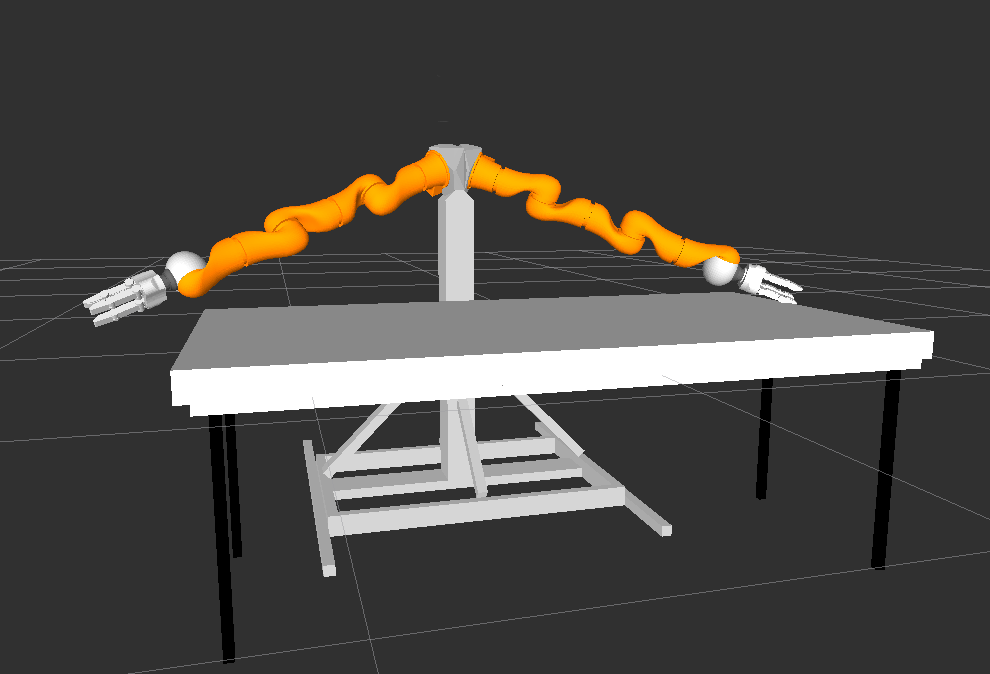
\includegraphics[width=0.75\textwidth]{images/iis_robot_table.png}
	\caption{URDF description in RViz}
	\label{fig:robot_table}
\end{figure}

\section{Creating the MoveIt configuration package}
\label{sec:moveit_assistant}

After designing the URDF description of our robot setup it was necessary to create a MoveIt configuration package. This was done, using the \emph{MoveIt Setup Assistant} which is part of the MoveIt distribution. This software tool provides a graphical user interface that allows to configure and generate a ROS package that contains all necessary MoveIt configuration files based on an existing URDF model. This section explains the steps that had to be performed and the resulting configuration package. \\ 

The Setup Assistant was launched using the following command line statement:
\begin{quote}
\begin{verbatim}
roslaunch moveit_setup_assistant setup_assistant.launch
\end{verbatim}
\end{quote}
This command brings up the Setup Assistant which asks for the file path to the previously created URDF description. After pointing the Setup Assistant to the correct file location, we had to perform the following configuration steps:

\begin{itemize}

\item \textbf{Computing the self collision matrix}

The \emph{self collision matrix} consists of pairs of robot links that can safely be excluded from collision checking. Adjacent links of the robot arm for example are in permanent collision. Collisions between other links can never happen because they are simply too far apart. The Setup Assistant can be triggered to compute this self collision matrix automatically by testing a large number of different robot configurations while tracking for link pairs that are hardly always in collision and pairs that are never in collision. The number of sample configurations to check can be adjusted. We selected the maximum possible density of 100.000 sample configurations to find as many colliding link pairs as possible. This is important because excluding a large number of link pairs raises performance during motion planning because collision checking is an expensive process. The resulting self collision matrix can be adjusted manually if necessary. The image in figure \ref{fig:self_col} shows a screenshot of this configuration step.

\begin{figure}[p]
	\centering
  	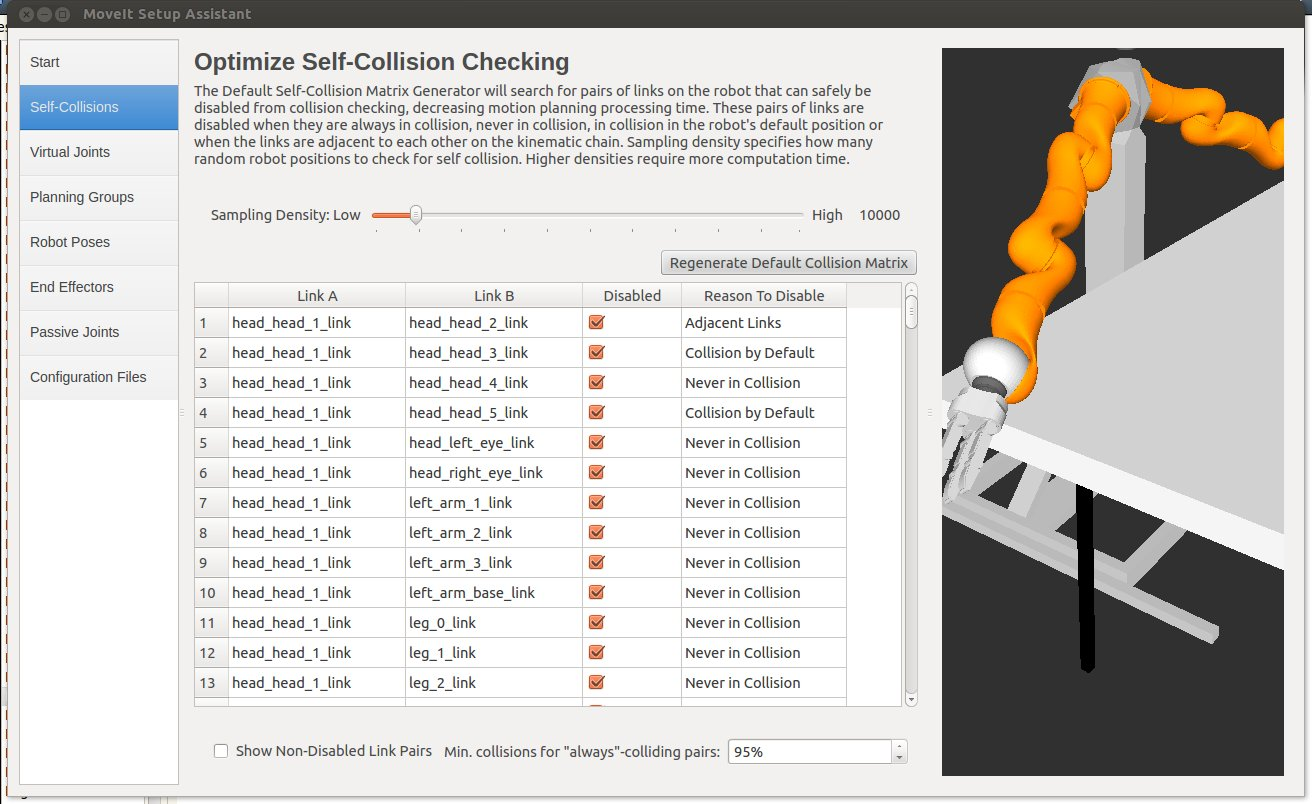
\includegraphics[width=0.75\textwidth]{images/self_collision.jpg}
	\caption{Computing the self collision matrix}
	\label{fig:self_col}
\end{figure}

\item \textbf{Defining the planning groups}

MoveIt requires to define so called \emph{planning groups} for the robot setup. A planning group is a group of links and joints within the model that can be seen as a logical component, e.g. a gripper or a robot arm. Each planning group consists of a unique name and a list of robot links and joints that are part of that group. Additionally can be specified, which IK solver should be used for the planning group.Each planning request in MoveIt is done against one of those defined planning groups. We defined planning groups for the both arms (\path{left_arm} and \path{right_arm}) and grippers (\path{left_sdh} and \path{right_sdh}). We decided to use the default KDL solver for the arms. An additional planning group, called \path{both_arms} was created that allows planning requests for both robot arms simultaneously. They were defined on the \emph{Planning Groups} page of the Setup Assistant (figure \ref{fig:planning_groups}).

\begin{figure}[p]
	\centering
  	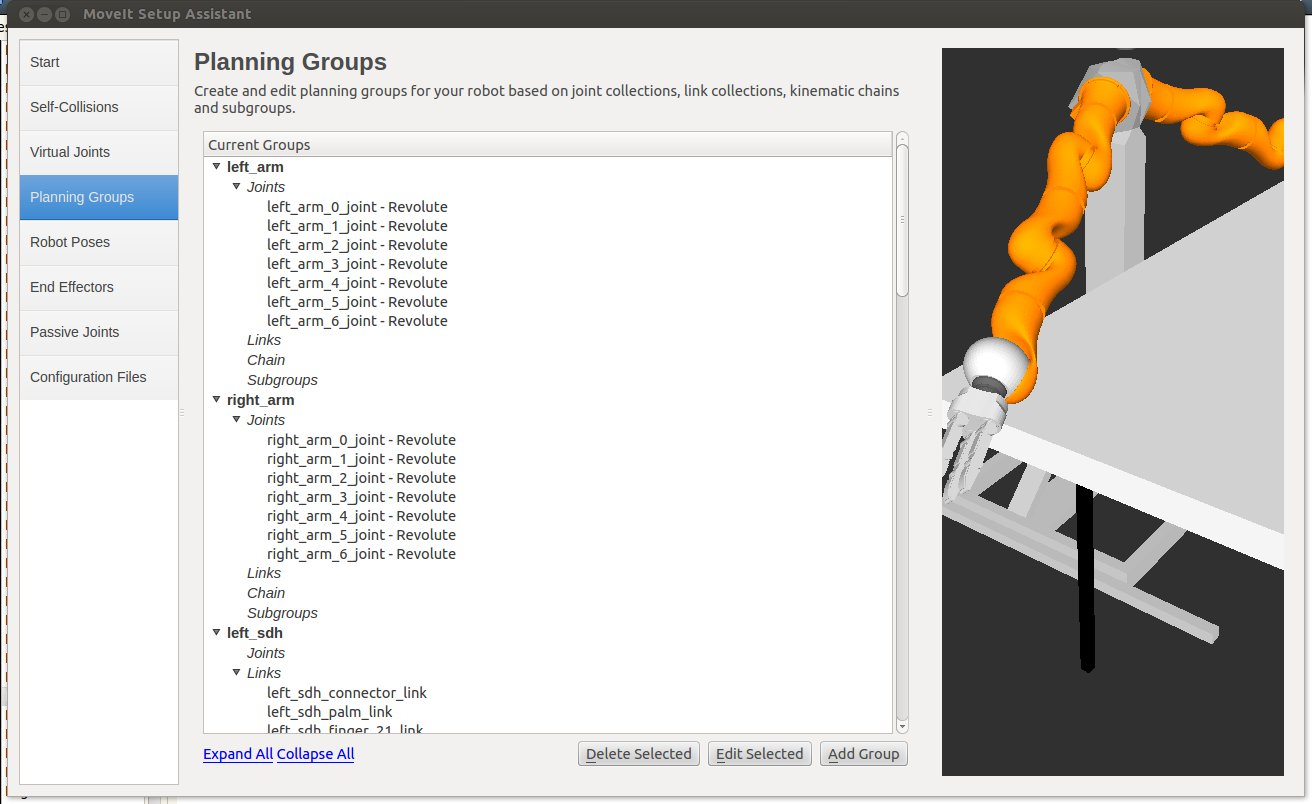
\includegraphics[width=0.75\textwidth]{images/planning_groups.jpg}
	\caption{Defining planning groups}
	\label{fig:planning_groups}
\end{figure}

\item \textbf{Defining the end effectors}

Each planning request in MoveIt requires to specify the end effector of the selected planning group. Those end effectors also had to be defined during the setup process. An end effector definition in MoveIt consists of a unique name, the underlying planning group (e.g. \path{left_sdh} or \path{right_sdh}), the parent planning group (e.g. \path{left_arm} or \path{right_arm}) and the name of the last link in the kinematic chain of the parent group. We defined end effectors as listed in table \ref{tbl:eef_defs}, using the \emph{End Effectors} page of the Setup Assistant.

\begin{table}[h]
  \centering
  \begin{tabular}[h]{|l|l|l|l|} \hline
	\textbf{Name} & \textbf{EEF group} & \textbf{Parent group} & \textbf{Parent link} \\ \hline
	\path{left_eef} & \path{left_sdh} & \path{left_arm} & \path{left_arm_7_link} \\
	\path{right_eef} & \path{right_sdh} & \path{right_arm} & \path{right_arm_7_link} \\ \hline
  \end{tabular}
  \caption{End effector definitions}
  \label{tbl:eef_defs}
\end{table}

\item \textbf{Completing the Setup Assistant}

The last step in the setup process was to generate a MoveIt configuration package based on the previously explained configuration steps. Therefore the Setup Assistant required to specify the desired package name which we set to \path{uibk_robot_moveit_config}. After triggering the package generation on the \emph{Configuration Files} page of the Setup Assistant, the resulting ROS package was created at the specified save location. 
 
\end{itemize}

The package that was generated during this setup process contains all the configuration and launch files that are necessary to make planning requests for our robot setup though it is not yet connected to the hardware. The configuration can be tested by running it in demo mode. This mode allows to plan and execute trajectories without being connected to the robot hardware. The demo mode is launched with the following command line statement:
\begin{quote}
\begin{verbatim}
roslaunch uibk_robot_moveit_config demo.launch
\end{verbatim}
\end{quote}
This command runs a \path{move_group} node using the previously created configuration and starts an instance of RViz with the motion planning plugin. There it is possible to switch between planning groups, set start and target configurations, do planning requests and visualize the resulting trajectories based on a graphical user interface. \\

The launch files within the configuration package are responsible for uploading the configuration parameters to the parameter server and start the \path{move_group} node. Those parameters are defined in several configuration files, located in the \path{config} folder of the configuration package. The following paragraphs just give an overview about content of the most important files. Detailed information can be found in the MoveIt documentation\footnote{http://moveit.ros.org/documentation/concepts/}.

\paragraph{\texttt{controllers.yaml}}
The content of this file specifies the available controllers for the (simulated or real) hardware. The file is initially empty and has to be populated manually. This was done after implementing the required controller interface, which is described in section \ref{sec:hardware_adapter}.

\paragraph{\texttt{fake\_controllers.yaml}}
This file is populated by the Setup Assistant and contains the definitions for the \emph{fake} controllers. The fake controllers simulate a connection to the hardware by providing the required ROS interface. They are used in demo mode to visualize the commanded robot motions in RViz. Each fake controller is defined by its name and a list, containing the names of the controlled robot joints.

\paragraph{\texttt{iis\_robot.srdf}}
This file contains all the semantic information about the robot that was configured during the setup process. The content is specified using the SRDF\footnote{http://wiki.ros.org/srdf} format. It holds the definitions of the configured planning groups, end effectors and the generated self collision matrix entries.

\paragraph{\texttt{joint\_limits.yaml}}
This file holds the velocity and acceleration limits of all joints contained in the robot description. The Setup Assistant creates the initial values based on the URDF model but this configuration file allows to specify other limits if necessary. MoveIt uses the limits that are configured within this file, not those configured in the URDF description. We used that option to drastically reduce the maximum allowed velocity of all arm joints to achieve slower robot motions.

\paragraph{\texttt{kinematics.yaml}}
This file contains the definition of the IK solvers that should be utilized for the robot arms. Currently we use the KDL kinematics plugin that is part of the MoveIt distribution. Additional parameters specify the default timeout value that is used for each IK calculation attempt and the maximum amount of iterations.

\paragraph{\texttt{ompl\_planning.yaml}}
This file holds OMPL specific configuration parameters. It defines the allowed planning algorithms for each planning group. We left the content of that file at its default values. \\

The configuration of this package can be adjusted either by editing the configuration files manually or by launching the Setup Assistant again. This can be done, using the \path{setup_assistant.launch} file from this package.

\section{Connecting MoveIt to the existing robot control interface}
\label{sec:hardware_adapter}

After creating the configuration package it was necessary to find a way to connect MoveIt to the (simulated or real) hardware to allow the execution of the planned trajectories. This section explains the necessary steps in detail. \\

The connection to the hardware happens via the \path{FollowJointTrajectory} action interface. This is a special kind of ROS interface that builds upon the \emph{ROS action protocol}\footnote{http://wiki.ros.org/actionlib/DetailedDescription}. Each robot component that is intended to be controlled by MoveIt has to provide this interface. The interface comprises of the following topics:
\begin{itemize}

\item \path{follow_joint_trajectory/goal}

This topic is used to send a \path{FollowJointTrajectoryActionGoal} message to the controller. This message describes a time parametrized trajectory that has to be executed along with allowed tolerance values for final joint positions and execution time. Those tolerances specify how precise the controller has to stick to the position, velocity, acceleration and time constraints defined for the trajectory in order to consider the execution to be successful.

\item \path{follow_joint_trajectory/feedback}

The controller uses this topic to continuously provide feedback about the current execution status. The feedback message contains information about the trajectory point the controller is currently processing.

\item \path{follow_joint_trajectory/result}

After finishing the trajectory execution the controller publishes the result to this topic. If the final joint positions lie within the specified tolerance values and the time constraints were met, the trajectory execution is considered to be successful. The message contains a status code and a status message.

\end{itemize}
The existing control interface of the robot components only allows to send joint target positions to the \path{joint_control/move} topic but without any time parametrization. So it was necessary to implement an additional ROS node that is capable of executing the generated trajectories, using the existing infrastructure. Therefore we utilized the functionality of the \path{ros_control} stack\footnote{http://wiki.ros.org/ros\_control}. Those packages allow to integrate and control robot hardware in a generalized way, facilitating the usage of existing controllers on different robots. The following section gives an overview about the \path{ros_control} stack.

\subsection{ROS control stack overview}

\begin{figure}[h]
	\centering
  	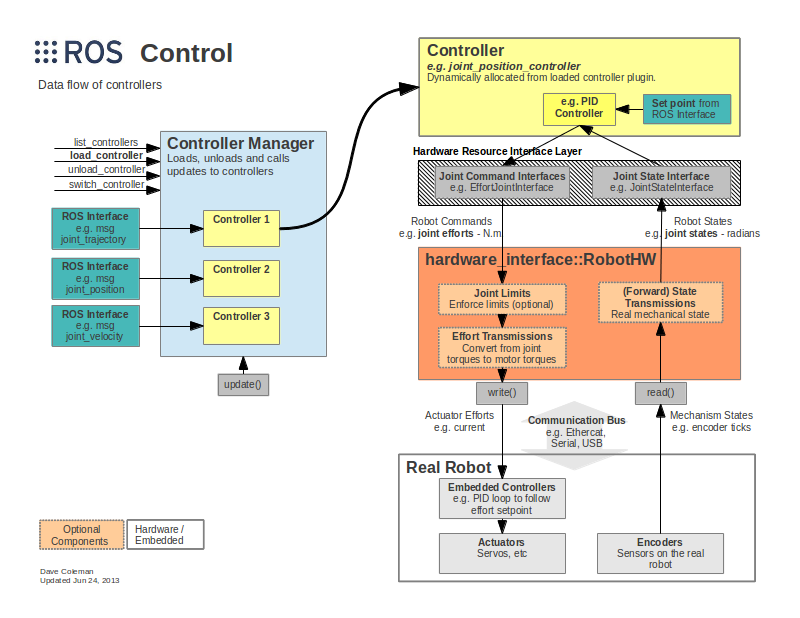
\includegraphics[width=1.0\textwidth]{images/ros_control.png}
	\caption{ROS control architecture}
	{\scriptsize Image source: http://wiki.ros.org/ros\_control}
	\label{fig:ros_control}
\end{figure}

A controller provides a ROS interface and translates the incoming control commands into suitable hardware commands. The ROS interface is controller specific and depends on how the robot is used. MoveIt for example requires controllers that provide the \path{FollowJointTrajectory} action interface, as explained above. The structure of the hardware commands depend on the available connection to the robot hardware. Some robots require commands that specify the target effort for the joint motors. Others, like our robot components allow to set joint target positions. The controllers are operated in a control loop which should run in real time. On each iteration of this control cycle the current state of the hardware is read. Then the controller calculates the control commands, based on the current state and the time since the last iteration. After that, the commanded values are sent back to the hardware and the next iteration starts. \\

Figure \ref{fig:ros_control} shows an overview about the \path{ros_control} architecture. The \path{ros_control} stack contains implementations for different kinds of generic hardware controllers. Within this project we utilized several \path{JointTrajectoryControllers}. This controller provides the \path{FollowJointTrajectory} action interface and calculates an interpolation between the trajectory waypoints that satisfies the velocity, acceleration and time constraints of the planned trajectory. The result are intermediate joint positions for each iteration of the control cycle that can be sent as target positions to the robot. The controller reads current hardware state like joint positions and velocities via the \path{JointStateInterface}. For writing the commanded values, the controller requires a \path{PositionJointInterface}. This interface simply allows to set a target position for a joint with a given name. Those interfaces are provided by the abstract \path{RobotHW} class which represents the connection to the hardware. Inheriting classes that represent a concrete robot have to register all the robot joints by their names (as configured in the URDF description), maintain their states and send commanded values back to the concrete hardware. \\

The controllers need to be registered on a \path{ControllerManager} instance. This class holds a reference to a \path{RobotHW} instance and provides an interface composed from ROS services that allows to load and start controllers for the connected hardware. The \path{LoadController} service forces a \path{ControllerManager} to load a controller with given name. It is necessary that a configuration for that controller is available on the parameter server that specifies the concrete controller type and controller specific details. After loading the controller it also needs to be started. This is done, using the corresponding \path{StartController} service. During the control cycle, the \path{ControllerManager} is responsible for updating all active controllers. \\

\subsection{Designing the hardware adapter node}

\begin{figure}[h]
	\centering
  	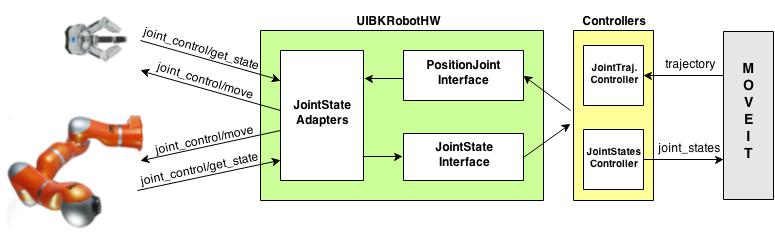
\includegraphics[width=1.0\textwidth]{images/hardware_adapter.jpg}
	\caption{Hardware adapter architecture}
	\label{fig:hardware_adapter}
\end{figure}

The \emph{hardware adapter} is an independent ROS node that we implemented to act as connection between MoveIt and the simulated or real hardware. The code and necessary configuration and launch files are located in the \path{uibk_moveit_adapter} package. The solution provides the necessary infrastructure for using generic controllers from the \path{ros_control} packages. Figure \ref{fig:hardware_adapter} gives an overview about the hardware adapter architecture. The \path{UibkRobotHW} is a subclass of \path{RobotHW} and represents the connection to the robot. It maintains the complete state of all joints in the connected robot components. Joints are represented by the \path{Joint} datatype, consisting of a unique joint name, state parameters and a commanded target position. For controllers, the \path{UibkRobotHW} class provides a \path{JointStatesInterface} and a \path{PositionJointInterface}. Active controllers use those interfaces to access the current state and for commanding target positions. \\ 

The \path{UibkRobotHW} utilizes a set of \path{JointStateAdapters}. A \path{JointStateAdapter} represents the connection to one specific robot component, e.g. a robot arm or a gripper. During the control cycle the \path{JointStateAdapters} read current joint states from the appropriate topics and send commanded values back to the hardware. Our solution allows to configure the utilized topic names via the parameter server.\\

On hardware adapter startup, an instance of the \path{UibkRobotHW} class is created and initialized by using the corresponding class method. It then searches the parameter server for the a parameter named \path{hardware_adapter/adapter_list}. This parameter specifies the names of the \path{JointStateAdapters} that need to be created. The \path{UibkRobotHW} class then creates a \path{JointStateAdapter} instance for each name it finds in the configured adapter list, based on the provided configuration settings. Listing \ref{lst:adapter_config} shows the current content of the corresponding configuration file (\path{adapter_config.yaml}). As the names of the topics that are used by the \path{JointStateAdapters} can be configured it becomes clear that the hardware adapter is able to interact with the simulator and the real robot as well, as both of them provide exactly the same ROS interface just within different namespaces. Available configuration parameters are:

\begin{itemize}

\item \textbf{\path{adapter_list}} \\
Contains a list of all \path{JointStatesAdapters} that have to be created. For each adapter name mentioned in this list a detailed configuration is required. The subsequent parameters have to be configured for each single adapter.

\item \textbf{\path{joint_state_topic}} \\
The name of the topic where a specific adapter listens for joint states. The expected message type  \path{sensor_msgs/JointStates}. This parameter is mandatory.

\item \textbf{\path{readonly}} \\
This parameter is optional. If true then the adapter will only listen for joint states but not publish commanded values.

\item \textbf{\path{joint_command_topic}} \\
The name of the topic the adapter should use to publish the commanded values to. The expected message type is \path{std_msgs/Float64MultiArray}. This parameter is mandatory if the adapter is not configured to be read only.

\item \textbf{\path{joints}} \\
A list of joint names that should be controlled by the adapter. The order in this list also determines the order of the values in the published message.

\item \textbf{\path{joint_name_prefix}} \\
This parameter can be used to be able to uniquely identify joints. For example both arms are using the same joint names (\path{arm_0_joint}, \path{arm_1_joint},\ldots). But in a URDF model, joint names have to be globally unique. Therefore the prefix can be used to prepend the original name to achieve uniqueness. A prefix value of \path{right_} for example will lead to the joint names \path{right_arm_0_joint}, \path{right_arm_1_joint},\ldots).

\end{itemize}

After instantiation, each \path{JointStateAdapter} waits a certain amount of time for a message containing the initial joint states on its configured joint states topic. If it does not receive such a message before timeout, it will automatically shut down for safety reasons and report an error. This is very important as the \path{JointStateAdapter} imediately begins to send joint positions after initialization. The position to be sent is initially the currently known position, as long as no other values have been commanded by the controllers. Therefore the initial position always has to be known, otherwise dangerous and rapid robot motions could occur on startup.

\begin{minipage}{\linewidth}
\lstinputlisting[caption={JointStateAdapter configuration}, label=lst:adapter_config]{code/adapter_config.yaml}
\end{minipage} \\

After the previously described initialization process a \path{ControllerManager} instance is created and the control loop is started. As the control loop must not be interrupted by ROS callback functions, it is launched in a separate thread. On each iteration the exact time since the last step is calculated. The \path{ControllerManager} is then forced to update all active controllers based on the time since last iteration. After handling the controllers, \path{JointStatesAdapters} are forced to send the commanded values to the hardware. This is done using the \path{publish} function of the \path{UibkRobotHW} class. Listing \ref{lst:control_loop} shows the code of the control loop thread.

\begin{minipage}{\linewidth}
\lstinputlisting[caption={Control loop thread}, label=lst:control_loop, style=customc]{code/control_loop.cpp}
\end{minipage} \\

It is important to note, that a running hardware adapter instance only provides the necessary infrastructure for \emph{using} controllers of the \path{ros_control} packages, not the controllers themselves. The required controllers still have to be loaded and started, using the corresponding ROS services of the \path{ControllerManager}. This has to be done after starting an instance of the hardware adapter node.

\subsection{Launching the hardware adapter}
\label{sec:launch_moveit}

This section describes how hardware adapter instances are launched for the simulator and the real robot, along with the arm and gripper controllers. \\

The file \path{hardware_adapter.launch}, located in the \path{uibk_moveit_adapter} package was created to handle the necessary configuration parameter upload and launch the hardware adapter node for the simulator and the real robot as well. As can be seen in listing \ref{lst:adapter_config} are the configured topic names for the \path{JointStateAdapters} defined, using \emph{relative} topic names (i.e. without trailing slash). The required instance is than accessed by simply shifting the node into \path{simulation} or \path{real} namespace. This is realized, specifying the \path{config_name} parameter of the launch file. The following command line statement launches a hardware adapter instance for the \path{simulation} namespace:
\begin{verbatim}
roslaunch uibk_moveit_adapter hardware_adapter.launch config_name:=simulation
\end{verbatim}

\lstinputlisting[caption={Launching the hardware adapter (\texttt{hardware\_adapter.launch})}, label=lst:adapter_launch]{code/hardware_adapter.launch}

Listing \ref{lst:adapter_launch} shows the content of this launch file. The \path{ns} argument of the \path{<group>} tag specifies the namespace for all nodes that are launched within that group. That means all relative topic names are prepended with the namespace, defined in the \path{config_name} attribute. A relative topic name of \path{left_arm/joint_control/move} for example results in the absolute topic name \path{/simulation/left_arm/joint_control/move}.\\

The controller configurations are located in separate files, namely \path{arm_controllers.yaml} and \path{gripper_controllers.yaml}. Listing \ref{lst:arm_controller} shows the controller configuration for the left and the right arm. The \path{type} parameter specifies the controller type. The \path{joints} parameter contains the names of the robot joints, the controller is responsible for. The section \path{constraints} describes controller specific tolerance values. The \path{goal_time} value defines the amount of time the controller is allowed to exceed the trajectory execution time to still consider the execution to be successful.

\lstinputlisting[caption={Configuration of arm controllers (\texttt{arm\_controllers.yaml})}, label=lst:arm_controller]{code/arm_controllers.yaml}

The launch file \path{controllers.launch} is responsible for uploading those configuration files to the parameter server and run the controllers. Listing \ref{lst:controllers} shows the content of this file. After uploading the content of the configuration files, all the controllers are loaded and started.
Utilized controllers are the previously described \path{JointTrajectoryController} and the \path{JointStateController}. The \path{JointStateController} publishes the collected states of all robot joints at once to the \path{joint_states} topic, which is used by the \path{move_group} node to monitor the current state of the robot. \\

\lstinputlisting[caption={Launching controllers (\texttt{controllers.launch})}, label=lst:controllers, style=customxml]{code/controllers.launch}

After a successful hardware adapter startup all the required controllers are available. The node provides feedback information about the state and errors during the startup process on the console output. It is crucial that the joint state topics of simulator or real robot are available before launching the hardware adapter node, otherwise it will not be able to work because of missing initial joint states. After successful startup, the additional controller topics can be found in the corresponding namespace.

\section{Adjusting the MoveIt configuration}

The prerequisites were now made for connecting MoveIt to the (simulated or real) robot. The last remaining step was to adjust the MoveIt configuration for establishing a connection to the \path{FollowJointTrajectory} controllers. Therefore we modified the configuration file \path{controllers.yaml} in the \path{uibk_robot_moveit_config} package. It contains a list, describing the controllers that are made available by the hardware adapter. Each controller description contains the name of the controller, its namespace, the controller type and a list, containing the names of the controlled joints.\\

For starting MoveIt we created the launch file \path{moveit_planning_execution.launch}. The aim of this file is to launch a fully configured \path{move_group} node either for simulated or real robot, together with the corresponding hardware adapter. The namespace can be selected using a boolean parameter named \path{simulation}. The following statement launches a MoveIt configuration, connecting the \path{move_group} instance to the real robot.
{\small 
\begin{verbatim}
roslaunch uibk_robot_moveit_config moveit_planning_execution.launch simulation:=false
\end{verbatim}}
The launch file also starts the RViz visualization tool configured with the motion planning plugin. This is used for visualizing the planned trajectories and can also be used to test the connection to the robot by making planning requests and execute the resulting trajectories.

\section{Testing the IK solver}

Solving the inverse kinematics problem is an important issue when working with the robot arms. Many planning algorithms depend on an IK solution for a given Cartesian space goal before they are able to solve planning problems. So we decided to test the quality of the KDL inverse kinematics solver that is used by MoveIt. As a side effect we were able to use the test results to visualize the area in the robot workspace that can be reached by the robot the arms. \\

\begin{table}[h]
  \centering
  \begin{tabular}[h]{|l|c|c|c|} \hline
	\textbf{Arm} & \textbf{Redundant IK} & \textbf{KDL solver} & \textbf{\%} \\ \hline
	Left arm & $10.392$ & $15.474$ & $+48.9$ \\
	Right arm & $10.025$ & $15.444$ & $+54.0$ \\ \hline
  \end{tabular}
  \caption{IK test results}
  \label{tbl:ik_results}
\end{table}

First we computed a test set, composed from 3.500 sample locations within the robot workspace. The sample points are uniformly distributed throughout the area that should be reachable by at least one of the robot arms. The offset between the samples is 10 cm in $x$, $y$ and $z$ direction. For each sample point we computed 17 different orientations. That resulted in a set, containing 59.500 sample poses. During testing we assumed those test poses to be end effector target positions. The test utilized MoveIt's IK functionality (KDL) to compute a valid joint configuration for each single sample pose and counted the positive results. This was done for each arm separately. The outcome was a set of sample poses, the solver was able to find valid solutions for. The same test was repeated, using the pre-existing IK solver that was already available for the IIS Lab robot setup. This solution is based on the method described by \citep{moore2010}. The test results are listed in in table \ref{tbl:ik_results} which shows the comparison between both tested IK solvers. The numbers in the columns 2 and 3 indicate the amount of positive IK calculation attempts for the sample poses contained in the test set. It can be seen that the success rate of the KDL solver is around $50 \%$ higher then the one of the pre-existing solution. \\

The IK calculation results of the KDL solver were then used to visualize the area that is reachable by the robot arms. This visualization can be seen in figure \ref{fig:ik_visualization}. Each colored dot indicates a location that can be reached by one or both robot arms. The dot color range is between green and red. Green dots are locations where the solver was able to find solutions for all 17 orientations. Red dots are locations with a low number of positive results, that means they are only reachable at certain end effector orientations. The images (a) and (b) show the combined results for both robot arms. Images (c) and (d) show the reachable area for the left and (e) and (f) for the right robot arm.

\begin{figure}[p]
	\centering
  	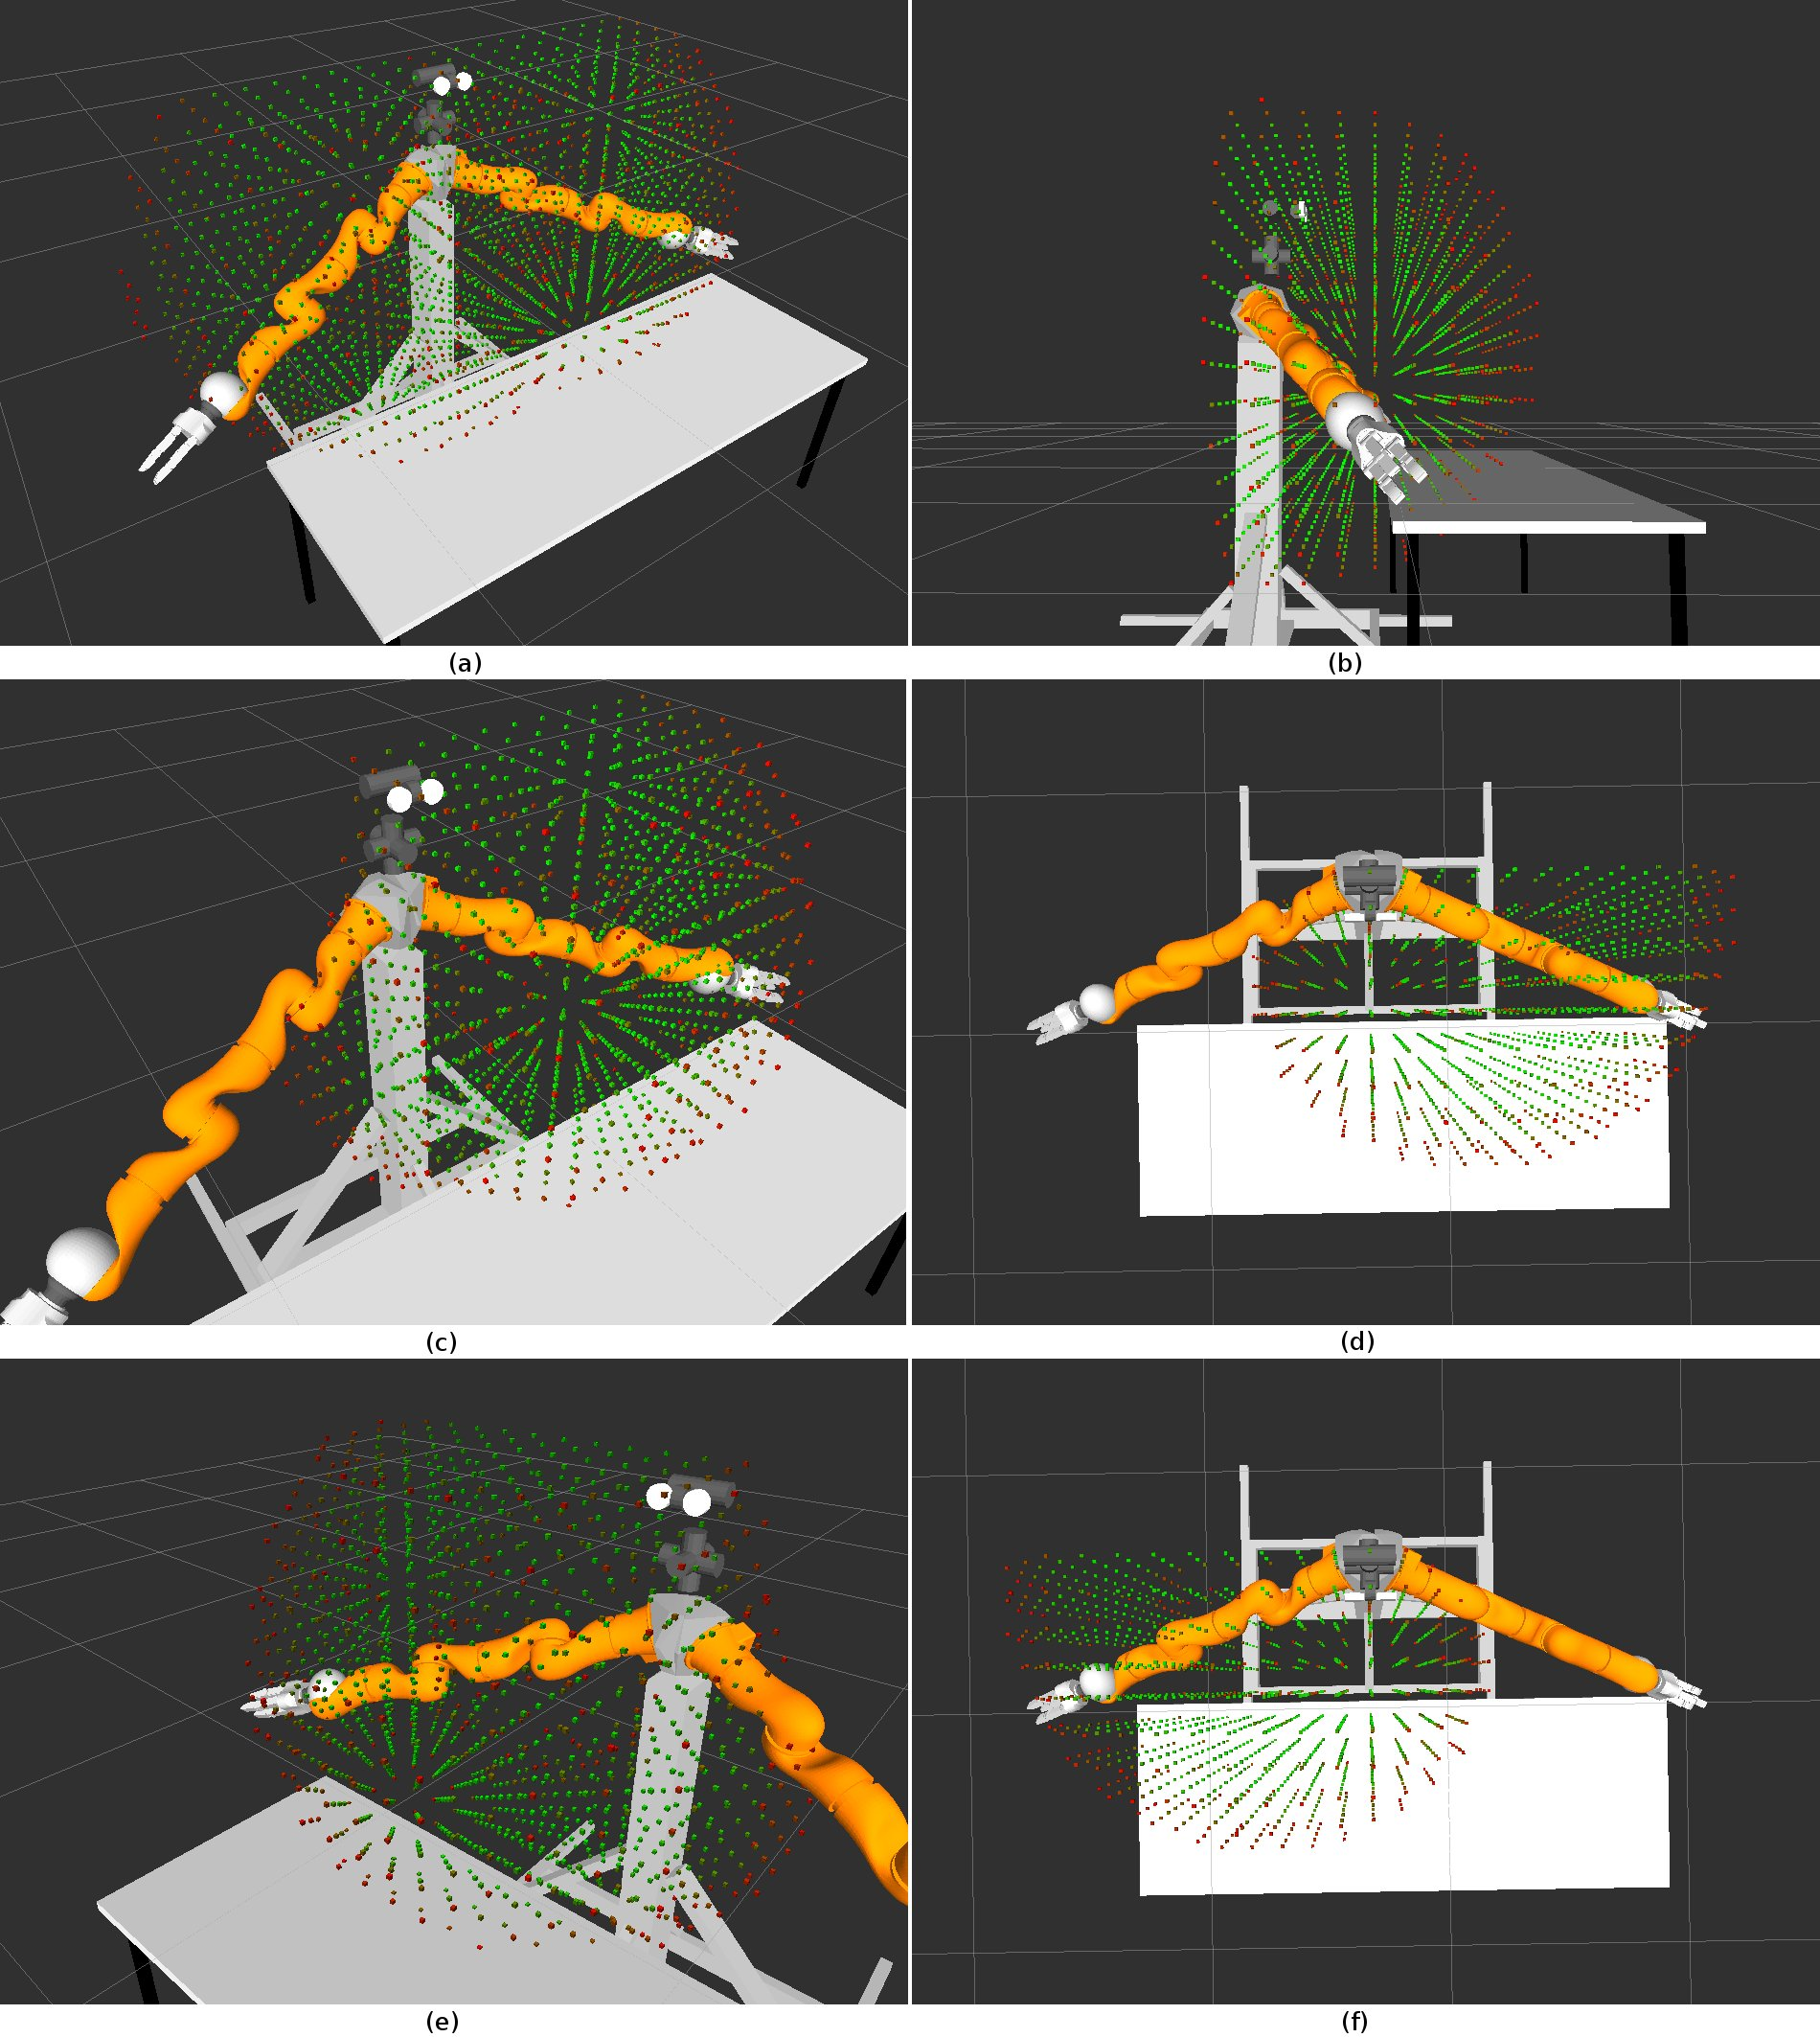
\includegraphics[width=1.0\textwidth]{images/results.jpg}
	\caption{IK test result visualization}
	\label{fig:ik_visualization}
\end{figure}

